% --- Chapter appendices, numbered <chapter>.A, .B, ... -----------------------
\renewcommand{\thesection}{\thechapter.\Alph{section}}
\setcounter{section}{0}

\section{Critical behaviour, small populations and conditional moments}
\label{m:app:criticalgw}

\Cref{m:sec:gw} defined the binary Galton--Watson process and
\cref{m:sec:extinction} settled whether it dies out. This appendix settles how, what
happens when it starts from more than one individual, and what the second moment of
the conditioned population does. The material is used in later chapters and referred
to from \cref{m:sec:overview,m:sec:condmeans}, but it is not needed to follow the
methods of \cref{m:sec:methods}, so it is collected here.

\subsection{The critical case: a power law and an infinite expected lifetime}
\label{m:app:critical}

At $p=\tfrac12$ the expectation is constant, $\ex{Z_n}=1$ for every $n$, and yet
extinction is certain by \cref{m:sec:extinction}. The two facts are reconciled by
the tail: rare realisations survive for enormously long times and grow enormously
large, and they do so at exactly the rate needed to hold the mean at one.

Let $T=\inf\{n:Z_n=0\}$ be the extinction time, so that the process passes through
generations $0,1,\dots,T-1$ and is dead at $T$. Writing $T$ as a sum of indicators
and taking expectations term by term --- legitimate because every term is
non-negative ---
\begin{equation}
\label{m:eq:ETsumSn}
\ex{T} = \sum_{n=0}^{\infty}\pr{T>n} = \sum_{n=0}^{\infty}\pr{Z_n>0}
= \sum_{n=0}^{\infty}S_n .
\end{equation}
Everything therefore turns on how fast $S_n$ decays at criticality, and that can be
established directly from the exact recursion.

\begin{proposition}[Critical survival probability]
\label{m:prop:criticalSn}
For the critical binary process, $p=\tfrac12$,
\begin{equation}
\label{m:eq:twoovern}
S_n\sim\frac{2}{n}\qquad(n\to\infty).
\end{equation}
\end{proposition}

\begin{proof}
At $p=\tfrac12$ the recursion \cref{m:eq:SnIter} reads
\begin{equation}
\label{m:eq:criticalrecursion}
S_{n+1} = S_n-\tfrac12S_n^2 = S_n\lrb{1-\frac{S_n}{2}} .
\end{equation}
By \cref{m:sec:extinction}, $S_n\downarrow0$, so the reciprocal sequence tends to
infinity. Its increments satisfy
\begin{equation}
\label{m:eq:reciprocalincrement}
\frac{1}{S_{n+1}}-\frac{1}{S_n}
= \frac{1}{S_n\lrb{1-\frac{S_n}{2}}}-\frac{1}{S_n}
= \frac{1}{2\lrb{1-\frac{S_n}{2}}}
\;\longrightarrow\;\frac12 .
\end{equation}
Summation of the convergent increments --- equivalently, the Stolz--Ces\`aro
theorem --- gives $(1/S_n)/n\to\tfrac12$, which is \cref{m:eq:twoovern}.
\end{proof}

Substituting into \cref{m:eq:ETsumSn}, the tail of the sum behaves like twice the
harmonic series,
\begin{equation*}
\ex{T} = \sum_{n=0}^{\infty}S_n\sim\sum_{n=1}^{\infty}\frac{2}{n},
\end{equation*}
which diverges (\cref{m:fig:harmonic}). Since every $S_n$ is positive,
$\ex{T}=\infty$: the expected lifetime of the critical Galton--Watson process is
infinite even though extinction occurs with probability one. The point
probabilities follow from the exact decrement in \cref{m:eq:criticalrecursion},
\begin{equation}
\label{m:eq:criticalTtail}
\pr{T=n+1} = S_n-S_{n+1} = \tfrac12S_n^2\sim\frac{2}{n^2} .
\end{equation}

\begin{figure}[H]
    \centering
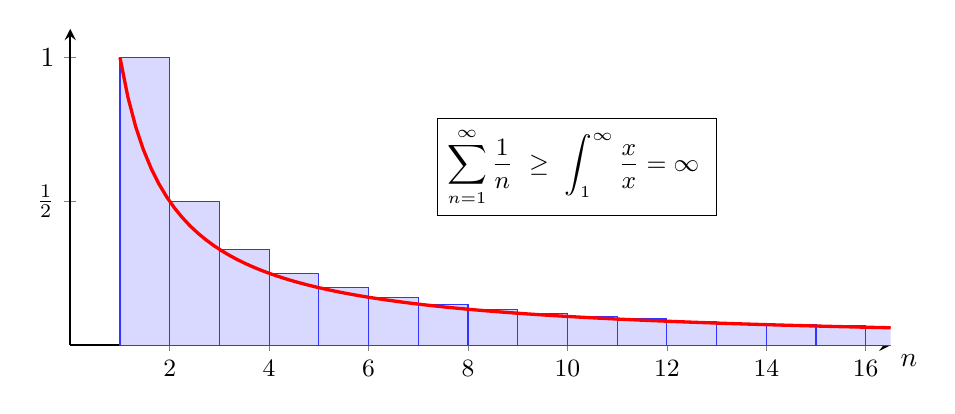
\begin{tikzpicture}
    \begin{axis}[
        axis lines = middle,
        xmin = 0, xmax = 16.5, ymin = 0, ymax = 1.1,
        xlabel = {$n$},
        xtick = {2,4,6,8,10,12,14,16},
        ytick = {0.5, 1}, yticklabels = {$\frac{1}{2}$, $1$},
        axis line style = {thick},
        width = 12cm, height = 5.6cm,
        every axis x label/.style={at={(current axis.right of origin)}, anchor=north west},
        xticklabel style={font=\small},
    ]
        \addplot[fill=blue!15, draw=blue!80, ybar interval, samples at={1,2,...,17}] {1/x} \closedcycle;
        \addplot[red, domain=1:16.5, samples=100, very thick] {1/x};
        \node[draw, fill=white, align=left, font=\small] at (axis cs: 10.2, 0.62) {
            $\displaystyle \sum_{n=1}^{\infty} \frac{1}{n} \ \ge\ \int_{1}^{\infty} \frac{\dd x}{x} = \infty$
        };
    \end{axis}
\end{tikzpicture}
\caption{Divergence of the harmonic series. Each blue rectangle has area $1/n$ and
contains the region under the red curve $1/x$ on $[n,n+1]$, so the sum of the areas
exceeds $\int_1^\infty x^{-1}\dd x=\infty$. Because $S_n\sim2/n$ at criticality,
the same divergence carries over to $\ex{T}=\sum_nS_n$.}
\label{m:fig:harmonic}
\end{figure}

The total progeny obeys a different exponent, and it can be computed exactly. Let
$\mathcal T = \sum_{n\ge0}Z_n$. A finite binary genealogy with $k$ division
vertices carries $k+1$ terminal vertices, hence $2k+1$ individuals in all, and the
number of ordered full binary trees with $k$ internal vertices is the Catalan
number $C_k = (k+1)^{-1}\binom{2k}{k}$. Each such tree is realised with probability
$p^k(1-p)^{k+1}$, so
\begin{equation}
\label{m:eq:totalprogenyexact}
\pr{\mathcal T = 2k+1} = C_k\,p^k(1-p)^{k+1},
\end{equation}
and $\pr{\mathcal T=2k}=0$. At $p=\tfrac12$, Stirling's formula applied to $C_k$
gives
\begin{equation}
\label{m:eq:totalprogenyasym}
\pr{\mathcal T = 2k+1}\sim\frac{1}{2\sqrt\pi}\,k^{-3/2},
\end{equation}
the classical $3/2$ law of critical branching, holding along the odd support.

The heavy tails responsible are visible directly in simulation. A power-law
distributed quantity carries a modest but non-negligible chance of an
extraordinarily large realisation, and a sample mean computed from such a quantity
does not settle: the larger the sample, the larger the mean, because the occasional
enormous value keeps pushing the normalised sum upward.

\begin{figure}[ht]
    \centering
    
\includegraphics[width=0.96\textwidth]{power_law_fixed.pdf}
    \caption{Power-law behaviour in the critical Galton--Watson process
    ($p=0.5$), from $10^6$ realisations.
    (a) Survival probability $S_n=\pr{Z_n>0}$, showing the late-generation scaling
    $S_n\sim2/n$ of \cref{m:eq:twoovern}.
    (b) Probability mass function of the extinction time $T=\inf\{n:Z_n=0\}$, with
    heavy tail $\pr{T=n}\sim2/n^2$.
    (c) Probability mass function of the total progeny
    $\mathcal T=\sum_{k\ge0}Z_k$, displaying the $n^{-3/2}$ asymptotic
    \cref{m:eq:totalprogenyasym} on its odd support.}
    \label{m:fig:power_law}
\end{figure}

\subsection{A continuum view of the survival recursion}
\label{m:app:riccati}

The critical asymptotic \cref{m:eq:twoovern} is also reachable by treating $n$ as
continuous, and the comparison is instructive because the same substitution is made
elsewhere in this thesis where it cannot be repaired so easily.

Once $n$ is large the unit generational increment is small compared with the scale
on which $S_n$ varies, so the difference on the left of
\cref{m:eq:criticalrecursion} may be replaced by a derivative:
\begin{equation*}
\dda{S}{n} = -\tfrac12S^2,
\qquad\text{with general solution}\qquad
S(n) = \frac{2}{n+\text{const}} .
\end{equation*}
This replaces a difference equation by a differential one, and nothing in the step
justifies the replacement beyond the smallness of the increment relative to the
solution. \Cref{m:prop:criticalSn} shows that the conclusion is nevertheless
correct.

Away from criticality the same substitution is less benign. With
$\varepsilon = 1-2p$ the recursion \cref{m:eq:SnIter} rearranges to
$S_{n+1}-S_n = -\varepsilon S_n-pS_n^2$, and the continuum replacement gives the
Riccati equation
\begin{equation}
\label{m:eq:riccati}
\dda{S}{n} = -\varepsilon S - pS^2 ,
\end{equation}
which the substitution $u=1/S$ linearises to $u' = \varepsilon u+p$, with solution
$u(n) = K\ee^{\varepsilon n}-p/\varepsilon$ and hence
\begin{equation}
\label{m:eq:riccatisol}
S(n) = \frac{\varepsilon}{K\varepsilon\,\ee^{\varepsilon n}-p} .
\end{equation}
Setting $\varepsilon=0$ recovers \cref{m:eq:twoovern}; keeping $\varepsilon>0$
recovers the geometric decay $S_n\sim A(p)(2p)^n$ of \cref{m:eq:Apdef}, since
$(2p)^n = \ee^{n\ln(1-\varepsilon)}$ agrees with $\ee^{-\varepsilon n}$ to leading
order. But the constant $K$ is fixed by the initial condition, that is by the early
generations, where the approximation is invalid; the continuum equation cannot
supply it. Since $K$ is precisely $A(p)$, this is the analytic statement of the
obstruction described in \cref{m:sec:dtlimit}: no argument of this kind will produce
the amplitude, and a different method is needed. \ChAcap{} supplies it.

Note that the same Riccati structure reappears in \cref{m:app:absbirthdeath} as the
characteristic equation of a partial differential equation, where it \emph{can} be
solved outright --- the difference being that there it is an exact consequence of
the model rather than a continuum approximation to a difference equation.

\subsection{Survival of small populations}
\label{m:app:smallpops}

Near criticality, with $p$ and $1-p$ each close to a half, a lineage dies at its
first round almost half the time. Should it survive one generation, both its
offspring fail at their own first attempt with probability around $0.25$, so the
lineage reaches the second generation only with probability about $0.375$:
\begin{equation*}
0.375\approx
\underbrace{(1-0.5)}_{\text{no extinction at the first step}}\times
\underbrace{(1-0.5\times0.5)}_{\text{nor at the second}} .
\end{equation*}
More generally, survival to a given generation is obtained by iterating
\cref{m:eq:SnIter}. At exactly critical branching the extinction probabilities for
$n=1,2,3,4$ are $u_n = 0.500,\ 0.625,\ 0.695,\ 0.741$ to three significant figures,
so the probability of survival decays quickly over the first few rounds, and does
so almost as fast just above criticality as just below. \Cref{m:fig:earlySn} makes
the point: whatever advantage supercriticality confers, it is not an
early-generation advantage.

\begin{figure}[ht]
\centering
  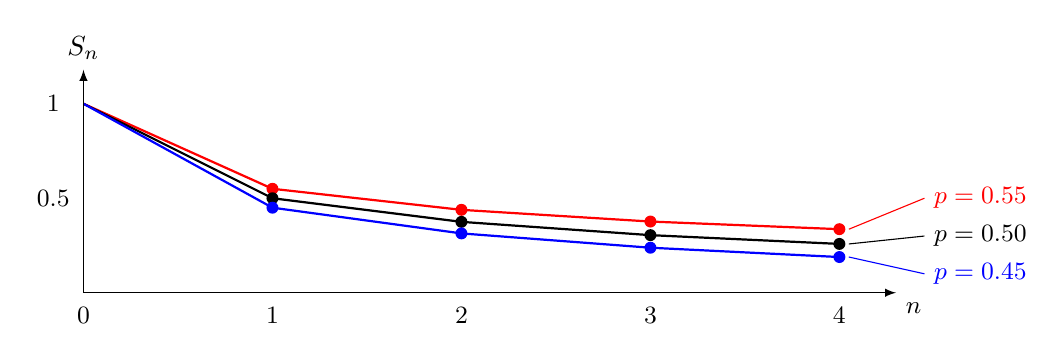
\begin{tikzpicture}[scale = 2.4]
    \foreach \x/\y/\color in {1/0.55/red, 2/0.4386250/red, 3/0.3766719/red, 4/0.336304/red,
                              1/0.5/black, 2/0.375/black, 3/0.3046875/black, 4/0.25827/black,
                              1/0.449999/blue, 2/0.313874/blue, 3/0.2381546/blue, 4/0.188816/blue}
      \fill[color=\color] (\x, \y) circle (0.9pt);
    \draw[red, thick] (0, 1) -- (1, 0.55) -- (2, 0.4386250) -- (3,0.3766719) -- (4,0.336304);
    \draw[black, thick] (0, 1)--(1,0.5) --  (2,0.375) -- (3,0.304687) -- (4,0.25827);
    \draw[blue, thick] (0, 1)--(1,0.449999)  --  (2,0.313874) -- (3,0.238154) -- (4,0.18881);
    \draw[-latex] (0,0) -- (4.3,0) node[below right, font=\small] {$n$};
    \draw[-latex] (0,0) -- (0,1.18) node[above] {$S_n$};
    \foreach \x/\lab in {0/0, 1/1, 2/2, 3/3, 4/4} \node[font=\small] at (\x, -0.12) {\lab};
    \foreach \y/\lab in {0.5/0.5, 1/1} \node[font=\small] at (-0.16, \y) {\lab};
    \draw[red,  thin] (4.05,0.336) -- (4.45,0.50);
    \draw[black,thin] (4.05,0.258) -- (4.45,0.30);
    \draw[blue, thin] (4.05,0.189) -- (4.45,0.10);
    \node[red,  font=\small, anchor=west] at (4.45, 0.50) {$p=0.55$};
    \node[black,font=\small, anchor=west] at (4.45, 0.30) {$p=0.50$};
    \node[blue, font=\small, anchor=west] at (4.45, 0.10) {$p=0.45$};
  \end{tikzpicture}
\caption{Survival probability over the first four generations from a single
progenitor. Even in the supercritical case ($p=0.55$) the early decay is steep, and
the three curves have barely separated by $n=4$.}
\label{m:fig:earlySn}
\end{figure}

\subsubsection*{An initial cohort of size \texorpdfstring{$k$}{k}}

Suppose now $Z_0=k$: the process begins with a group rather than an individual.
Under supercritical branching, growth becomes more predictably exponential as the
count rises, because a large number of individuals lets the expected dynamics show
through the noise. The founding cohort is precisely the regime in which that noise
dominates instead.

The lineages are independent and each is extinct by generation $n$ with probability
$u_n$, so all $k$ have gone with probability $u_n^{\,k}$ and
\begin{equation}
\label{m:eq:Snk}
S^{(k)}_n = 1-u_n^{\,k} .
\end{equation}
Letting $n\to\infty$ and using \cref{m:eq:Sinfty}, the ultimate establishment
probability is $0$ for $p\le\tfrac12$ and $1-\bigl((1-p)/p\bigr)^k$ for
$p>\tfrac12$: a larger cohort helps decisively above criticality and, in the long
run, not at all below it. \Cref{m:fig:kvals,m:fig:kvals2} show $S^{(k)}_n$ through
$500$ generations for $k=1,10,100,1000$. The improvement in longevity that a larger
first cohort buys is acutely sensitive to criticality, and the two panels of
\cref{m:fig:kvals2} differ only in the third decimal place of $p$.

\begin{figure}[ht]
\centering

\includegraphics[width=0.52\textwidth]{kvals.png}
\caption{Survival probability $S^{(k)}_n$ from \cref{m:eq:Snk} out to $500$
generations at exact criticality, $p=0.5$, for $k=1,10,100,1000$ (blue through to
red). A larger founding cohort buys longevity, but at criticality every curve is
still headed for zero.}
\label{m:fig:kvals}
\end{figure}

\begin{figure}[ht]
\centering

\includegraphics[width=0.44\textwidth]{kvals505.png}
\hfill

\includegraphics[width=0.44\textwidth]{kvals495.png}
\caption{As \cref{m:fig:kvals}, but with $p$ displaced slightly from criticality:
$p=0.505$ on the left (supercritical), $p=0.495$ on the right (subcritical). A
displacement of half a per cent separates curves that were nearly coincident in
\cref{m:fig:kvals}.}
\label{m:fig:kvals2}
\end{figure}

\subsubsection*{Conditioning and apparent early growth}

The conditioning of \cref{m:sec:condmeans} has a mirror image worth recording,
because it shows that the effect is not confined to the subcritical case.

Consider an ensemble of independent homogeneous birth--death processes, all with
the same constant rates, and retain only those still alive at some large time. The
retained subpopulation is automatically enriched for early rapid growth: a
realisation that grew quickly at the outset is far more likely to have escaped the
early extinction risk documented in \cref{m:fig:earlySn}, and so far more likely to
be in the retained set. No change in the underlying rates is required to produce the
enrichment, and the apparent slowdown that follows is not a slowdown at all but a
reversion to the mean. The effect is known as the \emph{push of the past}, and was
identified in a setting far from the present one, as an explanation for a
systematic pattern in longevity and diversity data \cite{Budd2018}.

That is the conditioning of \cref{m:sec:condmeans} seen from the other side. There a
subcritical process was conditioned on survival and its mean settled to $1/A(p)$
rather than decaying; here a critical or supercritical process is conditioned on
survival to a late time and its early growth appears inflated. In both cases the
conditioning, not the mechanism, does the work: the selection is performed on
trajectories after they have been generated, and the steep early decline of
\cref{m:fig:earlySn} is the source of the resulting bias.

\subsection{The limiting conditional variance}
\label{m:app:condvariance}

\Cref{m:sec:condmeans} quoted the limiting conditional variance
\cref{m:eq:condvar} without deriving it. The derivation is short, it uses only the
composition rule \cref{m:eq:gwcomposition}, and it is worth having, because the mean
of a distribution says nothing about whether the distribution itself is settling
down: a second moment that also stabilises is the least one should ask of a
population claimed to be quasi-stationary.

Write $\phi_n$ for the generating function of $Z_n$, so that $\phi_n=\phi\circ
\phi_{n-1}$, and recall from \cref{m:eq:pgfmoments} that $\phi_n'(1)=\ex{Z_n}$ and
$\phi_n''(1)=\ex{Z_n(Z_n-1)}$. For the binary law \cref{m:eq:pgfbinary} the
derivative of the offspring function is $\phi'(z)=2pz$, and that single fact makes
the chain rule collapse. Differentiating the composition once,
\begin{equation}
\label{m:eq:phinprime}
\phi_n'(z) = \phi'\bigl(\phi_{n-1}(z)\bigr)\,\phi_{n-1}'(z)
= 2p\,\phi_{n-1}(z)\,\phi_{n-1}'(z),
\end{equation}
which at $z=1$ recovers $\ex{Z_n}=2p\ex{Z_{n-1}}=(2p)^n$, since $\phi_{n-1}(1)=1$.
Differentiating \cref{m:eq:phinprime} again,
\begin{equation}
\label{m:eq:phinsecond}
\phi_n''(z)
= 2p\Bigl\{\phi_{n-1}'(z)^2 + \phi_{n-1}(z)\,\phi_{n-1}''(z)\Bigr\},
\end{equation}
so, writing $v_n=\phi_n''(1)$ and evaluating at $z=1$,
\begin{equation}
\label{m:eq:vnrecursion}
v_n = (2p)^{2n-1} + 2p\,v_{n-1},
\qquad v_0 = 0 .
\end{equation}
The recursion is linear and unrolls to a geometric sum,
$v_n=\sum_{k=1}^{n}(2p)^{n-k}(2p)^{2k-1}=(2p)^n\sum_{k=1}^{n}(2p)^{k-1}$, that is
\begin{equation}
\label{m:eq:factorialmoment}
\ex{Z_n(Z_n-1)} = (2p)^n\,\frac{1-(2p)^n}{1-2p},
\qquad\text{whence}\qquad
\ex{Z_n^2} = (2p)^n\lrb{1+\frac{1-(2p)^n}{1-2p}} .
\end{equation}
The check at $n=1$ is immediate: the right-hand side is $4p$, and $Z_1$ equals
$2$ with probability $p$ and $0$ otherwise.

Now condition. Subcriticality means $2p<1$, so $(2p)^{2n}$ is negligible beside
$(2p)^n$ at large $n$, and dividing \cref{m:eq:factorialmoment} by
$S_n\sim A(p)(2p)^n$ from \cref{m:eq:Apdef} gives
\begin{equation}
\label{m:eq:condsecondmoment}
\ex{Z_n^2\mid Z_n>0}
= \frac{\ex{Z_n^2}}{S_n}
\;\xrightarrow[n\to\infty]{}\;
\frac{1}{A(p)}\lrb{1+\frac{1}{1-2p}} ,
\end{equation}
the geometric factors cancelling exactly as they did for the mean in
\cref{m:eq:qsmean}. Both conditional moments therefore converge, and subtracting the
square of the first from the second gives \cref{m:eq:condvar}.

Two remarks are in order. The limit \cref{m:eq:condsecondmoment} is again a function
of $p$ and the single constant $A(p)$ alone, so the second moment adds no new
unknown --- the whole quasi-stationary description of the binary process runs
through one number, and that concentration of the difficulty into a single constant
is what \ChA{} sets out to analyse. And convergence of
two moments is not convergence of a law; it is consistent with the Yaglom limit of
\cref{m:def:qsd} and corroborates it, but the limit itself is taken from the
literature cited there rather than established here.

\subsection{The discrete rupture calculation}
\label{m:app:discreterupture}

\Cref{m:rem:notmeanfield} asserted that a state-dependent catastrophe does not
reduce to a mean-field hazard. The elementary calculation behind that assertion is
recorded here; it is retained as a bridge to the birth--death--catastrophe models
of later chapters, not as a theory of them.

Let $\kappa$ be the probability that a given individual initiates catastrophe at a
step. A single individual fails to do so with probability $1-\kappa$, and a cohort
of size $N$ with $(1-\kappa)^N$.

\subsubsection*{Birth and catastrophe alone}

With no death, the census is known with certainty: from a single progenitor the
population doubles at each step prior to catastrophe. The total exposure over
generations $0,\dots,n-1$ is $1+2+\cdots+2^{n-1} = 2^n-1$, so the probability of
surviving to generation $n$ is
\begin{equation}
\label{m:eq:bdcS}
S_n = \prod_{i=0}^{n-1}(1-\kappa)^{2^i}
= (1-\kappa)^{\sum_{i=0}^{n-1}2^i}
= (1-\kappa)^{2^n-1} .
\end{equation}
The conditional probability of rupture at step $n$ itself, given that every earlier
step was passed, is
\begin{equation}
\label{m:eq:bdchalt}
1-(1-\kappa)^{2^{\,n-1}},
\end{equation}
$2^{n-1}$ being the number exposed at that step. \Cref{m:eq:bdchalt} is a
conditional probability and should not be confused with the unconditional
probability of the process ending at step $n$.

\subsubsection*{Death included}

Once death is allowed the census is random, and \cref{m:eq:bdcS} is replaced by the
exact but implicit \cref{m:eq:norupture}, in which the cumulative exposure
$H_n = \sum_{i=0}^{n-1}\widetilde Z_i$ appears inside an expectation. The natural
simplification replaces $H_n$ by its mean,
\begin{equation}
\label{m:eq:bdcguess}
S_n\overset{?}{=}(1-\kappa)^{\ex{H_n}},
\qquad
\ex{H_n} = \sum_{i=0}^{n-1}(2p)^i
= \begin{cases}
\dfrac{1-(2p)^n}{1-2p}, & p\neq\tfrac12,\\[8pt]
n, & p=\tfrac12,
\end{cases}
\end{equation}
and by the Jensen argument of \cref{m:rem:notmeanfield} this is a lower bound rather
than an identity. Nor are the steps independent, since passing one is evidence of a
smaller population and so raises the chance of passing the next; both effects push
the estimate the same way.

\subsubsection*{The exact object}

The bound is crude, but nothing forces one to stop there: the quantity
\cref{m:eq:norupture} has an exact closed recursion, and it is the marked
generating function that \cref{m:rem:notmeanfield} called for. Define
\begin{equation}
\label{m:eq:catweightedpgf}
F_n(s) = \ex{s^{\widetilde Z_n}(1-\kappa)^{H_n}},
\qquad F_0(s) = s ,
\end{equation}
which carries the population and its accumulated exposure jointly, the first in the
variable $s$ and the second in the weight. Condition on what the founder does at the
first step. It dies with probability $1-p$, contributing nothing further; it divides
with probability $p$, after which the two daughter lineages evolve independently and
each contributes a factor $F_n$; and either way the founder itself is exposed for one
step, contributing $1-\kappa$. Hence
\begin{equation}
\label{m:eq:catweightedrec}
F_{n+1}(s) = (1-\kappa)\,\phi\bigl(F_n(s)\bigr)
= (1-\kappa)\bigl(1-p+p\,F_n(s)^2\bigr) ,
\end{equation}
a functional iteration of exactly the type of \cref{m:eq:gwcomposition}, differing
from it only by the constant factor the exposure contributes at each step.

Two evaluations carry the quantities of interest. $F_n(1)$ is
\cref{m:eq:norupture}, the probability of no catastrophe in the first $n$ steps; and
$F_n(1)-F_n(0)$ is the probability of being both unruptured and non-extinct at
generation $n$, the joint event for which \cref{m:rem:notmeanfield} observed that
Jensen supplies no bound at all. Since \cref{m:eq:catweightedrec} is exact and costs
one composition per generation to iterate, it is the object to use whenever
\cref{m:eq:bdcguess} is too crude --- which is the honest position: the elementary
estimate is indicative, and the recursion is what replaces it.
